% Use class option [extendedabs] to prepare the 1-page extended abstract.
\documentclass[extendedabs]{bmvc2k}
\usepackage[colorlinks = true,
            linkcolor = blue,
            urlcolor  = blue,
            citecolor = blue,
            anchorcolor = blue]{hyperref}
\usepackage{kotex}
% for the fancy \koTeX logo
\usepackage{kotex-logo}
\usepackage{mathtools}  % brings in amsmath, also some improvements
\usepackage{amssymb} % brings in amsfonts, incl \square
% Document starts here
\usepackage{graphicx}
\begin{document}


\title{CAM and Grad-CAM final report}
\addauthor{
Taehun Kim$^{1}$
}{}{1}

\addinstitution{
$^1$ Department of Computer Science and Engineering, Pusan National University.  
}
 

\maketitle
\noindent

\section{Introduction}
Class Activation Mapping(CAM)\cite{cam} modifies image classification CNN architectures replacing fully connected layers with global average pooling and a $1\times1$ convolutional layer for visual explanation.
 
In contrast, Gradient-weighted Class Activation Mapping(Grad-CAM)\cite{gradcam} is the technique for producing visual explanations, without modifying the CNN architecture or re-training the model.

In this report, We implemented the CAM\cite{cam} and GradCAM\cite{gradcam} architecture, and test and analyze the result.

\begin{figure}[t]
\centering
	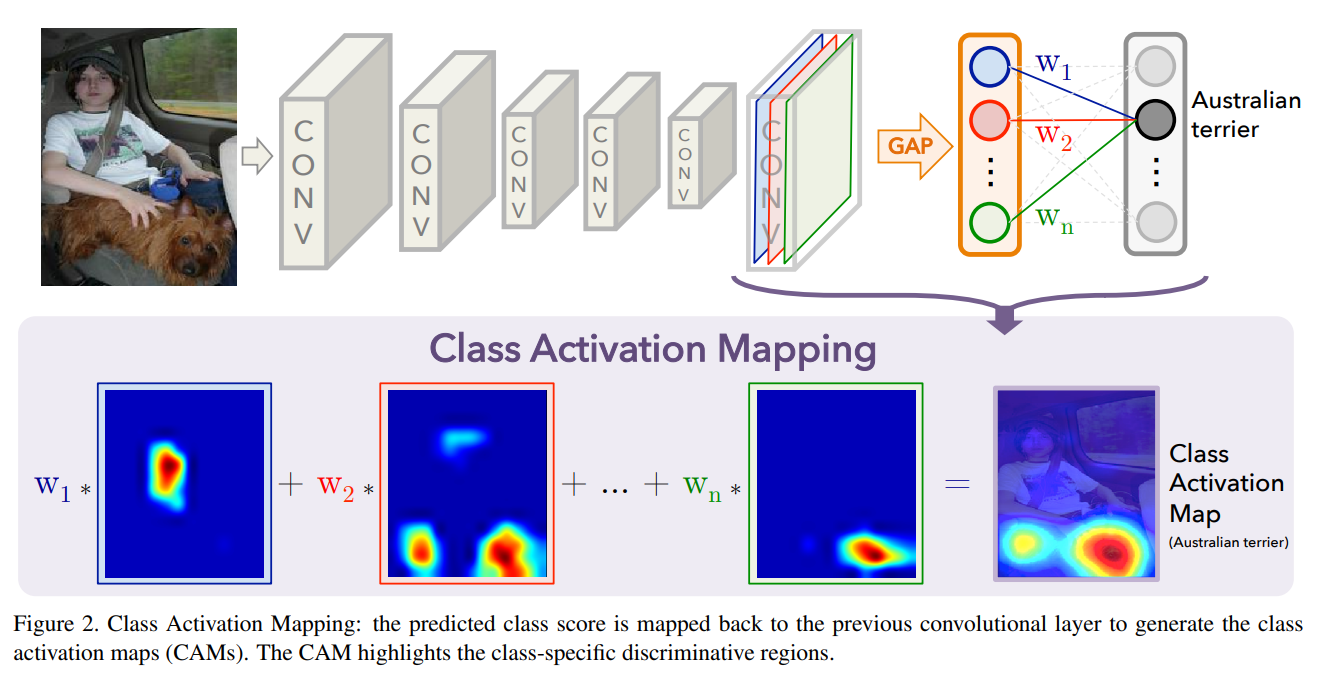
\includegraphics[width=\linewidth]{images/cam.PNG}
	\caption{
		Class Activation Mapping: the predicted class score is mapped back to the previous convolutional layer to generate the class.}
	\vspace{-2mm}
        \label{fig:cam overview}
\end{figure}

\begin{figure}[t]
\centering
	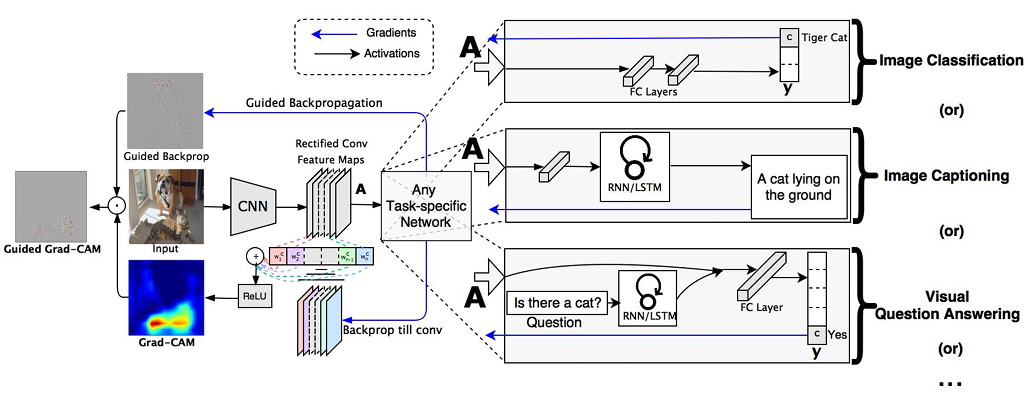
\includegraphics[width=\linewidth]{images/fig1.PNG}
	\caption{
		Grad-CAM overview}
	\vspace{-2mm}
        \label{fig:gradcamoverview}
\end{figure}
\section{CAM}
We use CIFAR-10 dataset for training, and we use the pretrained AlexNet\cite{alexnet} and pretrained VGG-13\cite{vggnet}. We removed the layers after last maxpooling layer, and we add $ 3\times 3 $ convolutional layers with 10 output channels, which we call \textit{cam-conv}.

After that, we add a global average pooling layer to each CNN, and we add a fully-connected layer with 10 output. Global average pooling refers to applying average pooling to the last convolutional layer, reducing its shape from $H\times W\times C$ to $1\times 1\times C$:
$$
F_k = \sum_{x,y} f_k(x,y)
$$

After training, we compute a weighted sum of those feature maps to produce CAM:

$$
M_c(x,y) = \sum_{x,y} w^c_kf_k(x,y)
$$
, where $M_c$ is class activation map for class c, and $w^c_k$ is the fully connected layer's weight parameters corresponding to specific output class c for unit k.
\subsection{Training}
As mentioned earlier, we use the CIFAR-10 dataset. The images are resized to $32\times32$ to $224\times224$ because $32\times32$ resolution of CIFAR-10 is too small for multiple max-pooling layers to be effectively applied. Additionally, we applied random horizontal flipping to the training images with a 50\% probability for data augmentation. Finally, all images were normalized with a mean of 0.5 and a standard deviation of 0.5.

We trained AlexNet using two different approaches: as a fixed feature extractor and with fine-tuning. In the first method, the convolutional layers are initialized with pretrained ImageNet weights to extract features, while the final classifier is trained for the new dataset. In the second method, not only is the classifier replaced or retrained, but the weights of the pretrained layers are also fine-tuned.

The learning rate for the first method is set to 0.001, while for the second method, it is 0.0001. Both methods were trained for 150 epochs. The results are shown in Table \ref{tab:camresult}.

\begin{table}[]
\centering
\begin{tabular}{|l|l|l|}
\hline
              & fixed feature extractor & fine-tuning \\ \hline
Test accuracy & 79.92\%                 & 90.02\%     \\ \hline
\end{tabular}
\caption{ The test accuracy of alexnet-cam model}
\label{tab:camresult}
\end{table}

\subsection{Analyze and Discuss}
AlexNet with fine-tuning performs better than when used as a fixed feature extractor. This is because the pretrained weights are initialized with ImageNet weights, while CIFAR-10 images have a lower resolution compared to ImageNet. As a result, the fixed feature extractor may struggle to extract features effectively from CIFAR-10 images.

Class Activation Maps of several CIFAR-10 images using a weighted sum of those feature maps are shown in Figure \ref{fig:camresult}

\section{Grad-CAM}
The last convolutional layer in a CNN has the best compromise between high-level semantics and spatial information. Grad-CAM uses the gradient information flowing into the last convolutional layer of the CNN. 
This method identifies the regions that contributed to the CNN's decision-making process.

Let activation maps of last convolutional layer is $A \in \mathbb{R}^{H\times W\times K}$, which $H\times W$ is resolution of the activation map and $K$ is the number of the activation maps. Let $y^c$denote the class score for class c before the softmax activation. First, The paper computes gradient of class score $y^c$ with respect to the $k$th map, $i$th column, $j$th row of $A$. Second, we apply global average pooling to the gradient to get the gradient of class score $y^c$ with respect $k$th $A$, $\alpha_k^c$:

$$ \label{exp:gradientavgpooling}
\alpha_k^c = \frac{1}{HW}\sum_{i=1}^W \sum_{j=1}^H \frac{\partial y^c}{\partial A^k_{ij}}
$$
, where the $A^k_{ij}$ is the $k$th map, $i$th column, $j$th row of activation maps of the last convolutional layer. Since $A$ is the last convolutional layer, the gradient calculation involves successive matrix multiplications of the weight matrices and the gradient with respect to activation from class score to last convolutional layer through Backpropagation(chain rule). $\alpha_k^c$ captures the importance of $k$th feature map for a target class c.

Additionally, we calculate localization map for class c using $\alpha_k^c, A^k,$ and ReLU:
$$
L^c_{Grad-CAM} = ReLU(\sum_k \alpha_k^c A^k)
$$
The product of $\alpha_k^c$ and $A^k$ highlights the significant regions within the activation map $A^k$.
ReLU is applied to retain only features with positive contributions, as negative values likely correspond to other classes.

$$
\text{ReLU}(x) =
\begin{cases} 
0 & \text{if } x \leq 0, \\
x & \text{if } x > 0.
\end{cases}
$$

\subsection{Implement and Result}
We use AlexNet\cite{alexnet} and VGG-16\cite{vggnet} with initalized with pretrained weight. To preserve the last convolutional layers'gradient($\frac{\partial y^c}{\partial A^k_{ij}}$) during backpropagation, we use register-hook function:
$$
\textbf{features} = \textbf{self.featureLayers(x)}
$$
$$
\textbf{features.registerHook(self.saveGradient)}
$$
, where featureLayers extract the feature from an image, and saveGradient function store the gradient to self.gradient and return the gradient.

To generate Grad-CAM, we compute the gradient with respect to the specified class probability ($y^c$). The gradient is stored in self.gradient and processed using global average pooling to obtain the averaged weights, $\alpha_k^c$. 

These weights are then used to compute a weighted sum of the activation maps($A^k$) to produce the class activation map. Finally, weighted sum of the activation maps is resized to the size of the original image for visualization. The visualization of Grad-CAM is shown in \ref{fig:gradcamresult}.
\section{Conclusion}
We implemented CAM\cite{cam} and Grad-CAM\cite{gradcam}. Through CAM and Grad-CAM, we were able to identify which parts of the image the CNN model focuses on(see Figure \ref{fig:camresult} and Figure \ref{fig:gradcamresult}). However, Grad-CAM is better because it does not require modifying the CNN model architecture or additional training.

\begin{figure}[t]
\centering
	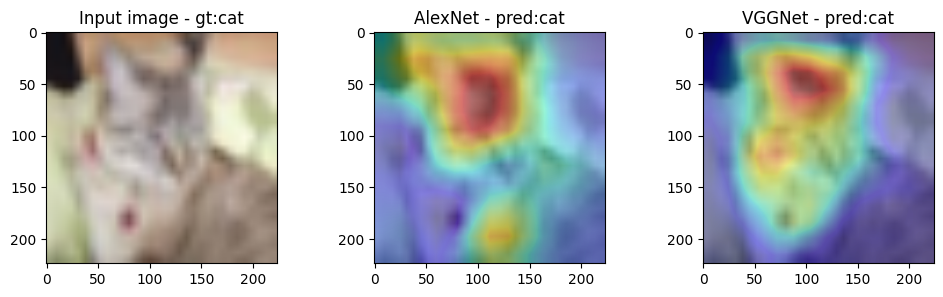
\includegraphics[width=\linewidth]{images/camresult1.png}
    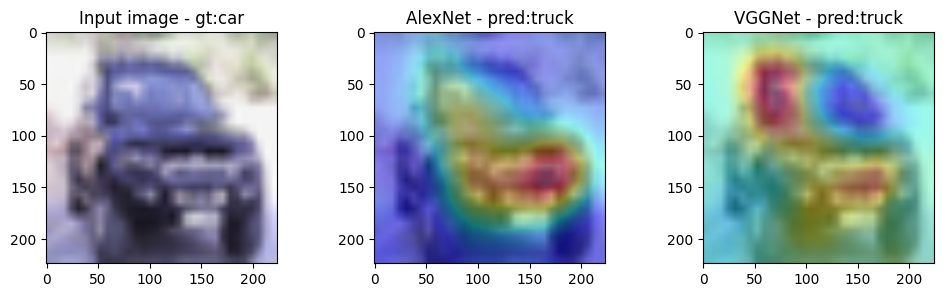
\includegraphics[width=\linewidth]{images/camresult2.png}
    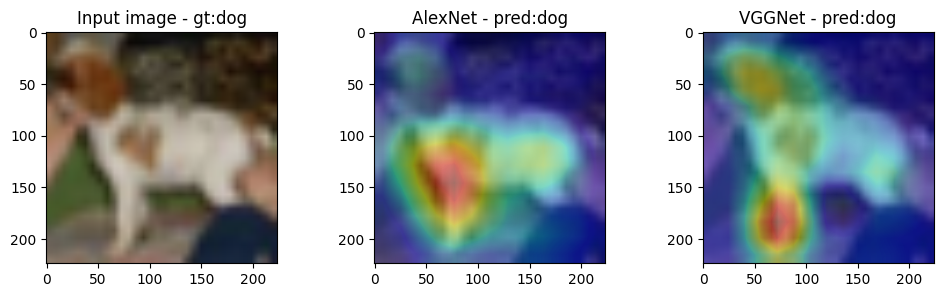
\includegraphics[width=\linewidth]{images/camresult3.png}
    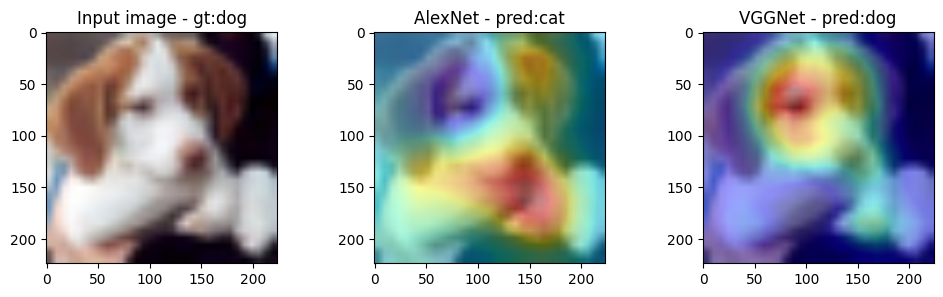
\includegraphics[width=\linewidth]{images/camresult4.png}
    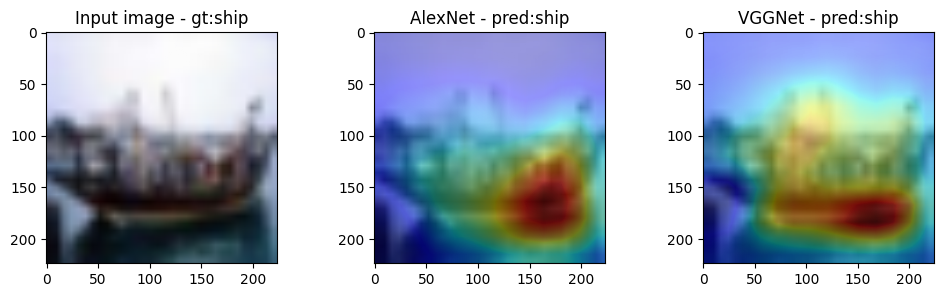
\includegraphics[width=\linewidth]{images/camresult5.png}
	\caption{
		Class Activation Map result of several CIFAR-10 images. The red areas indicate the parts of the image that the model paid more attention to.}
	\vspace{-2mm}
        \label{fig:camresult}
\end{figure}

\begin{figure}[t]
\centering
	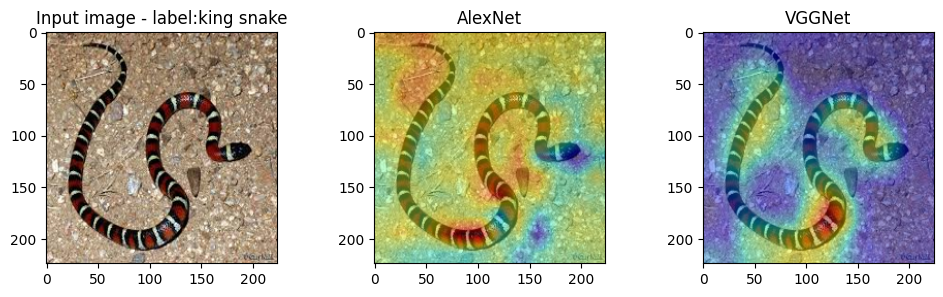
\includegraphics[width=\linewidth]{images/gradcamresult1.png}
    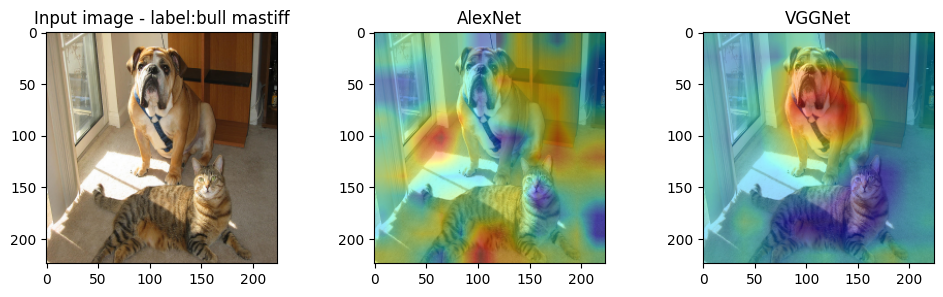
\includegraphics[width=\linewidth]{images/gradcamresult2.png}
    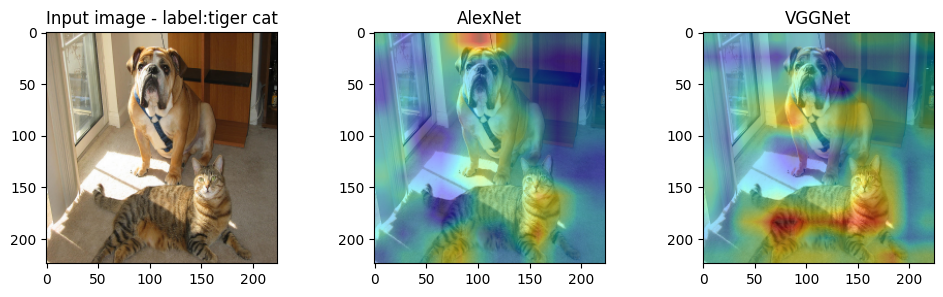
\includegraphics[width=\linewidth]{images/gradcamresult3.png}
    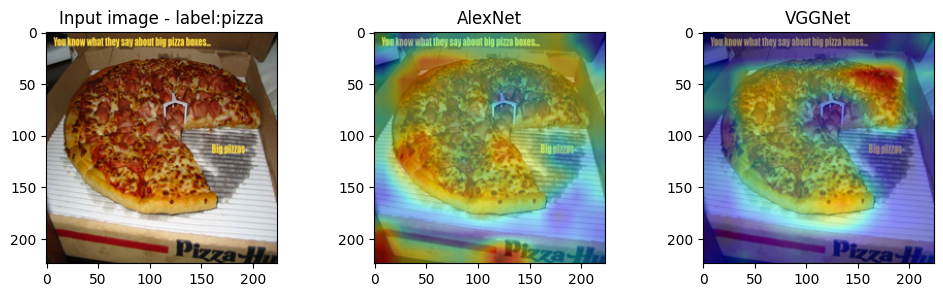
\includegraphics[width=\linewidth]{images/gradcamresult4.png}
    
	\caption{
		Grad-CAM results of several images. The red areas indicate the parts of the image that the model paid more attention to. }
	\vspace{-2mm}
        \label{fig:gradcamresult}
\end{figure}

\newpage
\bibliography{egbib}

\end{document}
